\section{Evaluation}
\label{sec:evaluation}

We evaluate \scout with three sets of big data analytics
applications on 18 cloud configurations on a single-node.
We further evaluate 69 cloud configuration on multiple nodes.
Our evaluations show that \scout finds the optimal or near-optimal configuration more often than other methods
and does so while reducing search costs.

\subsection{Experiment Setup}
\label{sec:setup}

\subsubsection*{Workloads}
We choose diverse workloads (CPU-intensive, memory-heavy, IO-intensive and network-intensive) such as PageRank, sorting, recommendation, classification and online analytical processing (OLAP).
We also change the input parameters and data sizes to create
a wide spectrum of workloads. 
These workloads run on Apache Hadoop~\cite{hadoop} and two separate versions of Apache Spark~\cite{spark} (version 1.5 and 2.1). 

\begin{figure}[!htbp]
\centering
\begin{subfigure}[b]{0.4\textwidth}
    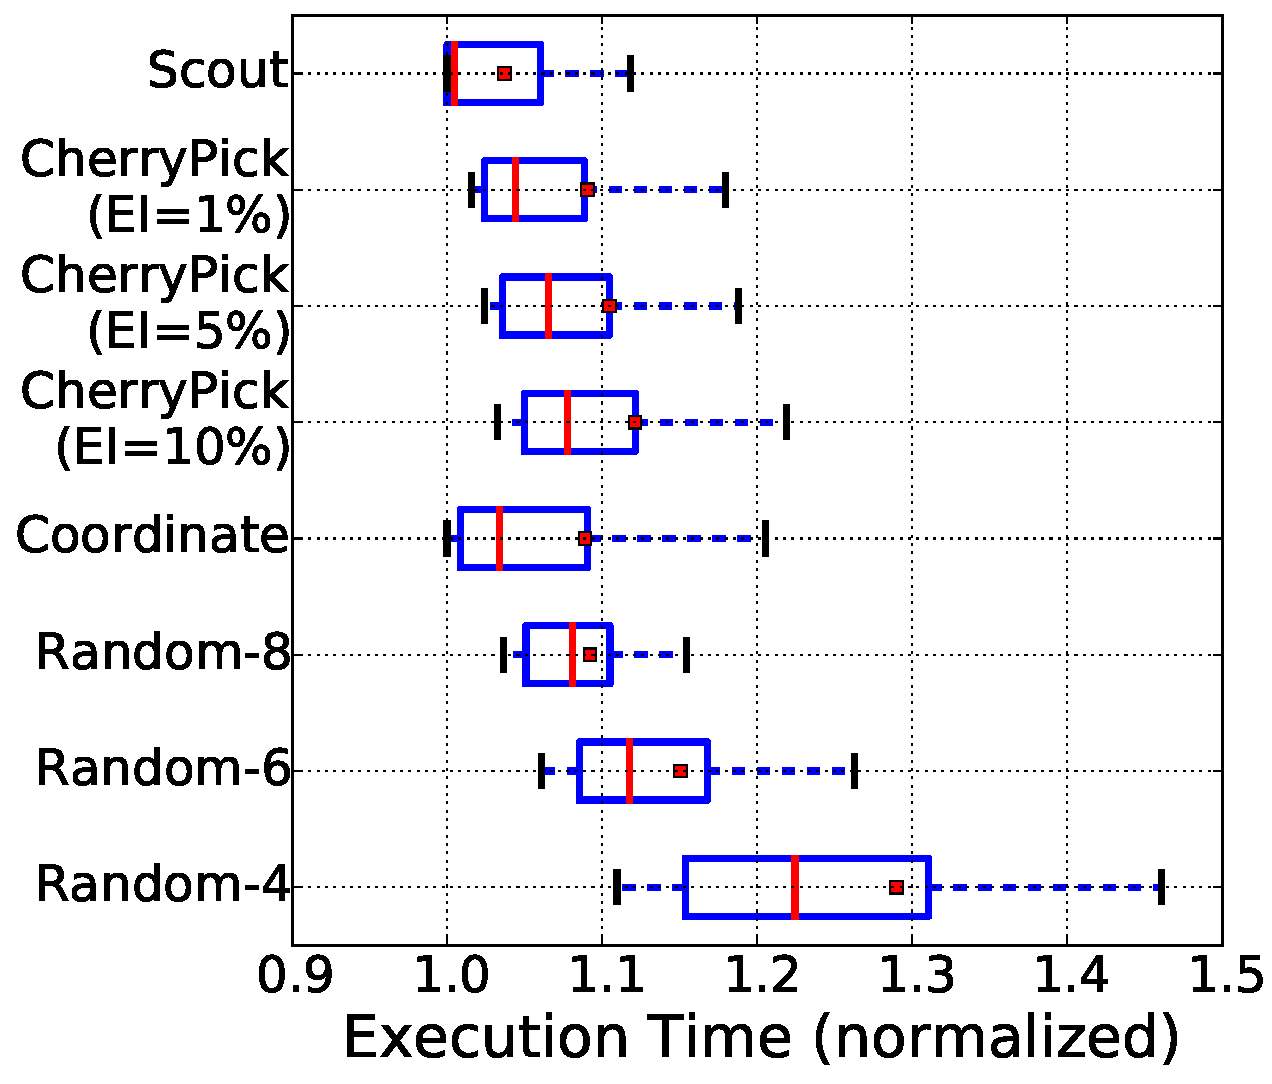
\includegraphics[width=\linewidth]{figures/single_time_overall_performance.pdf}
    \caption{Search Performance}
    \label{fig:single_time_overall_performance}
\end{subfigure}
\begin{subfigure}[b]{0.4\textwidth}
    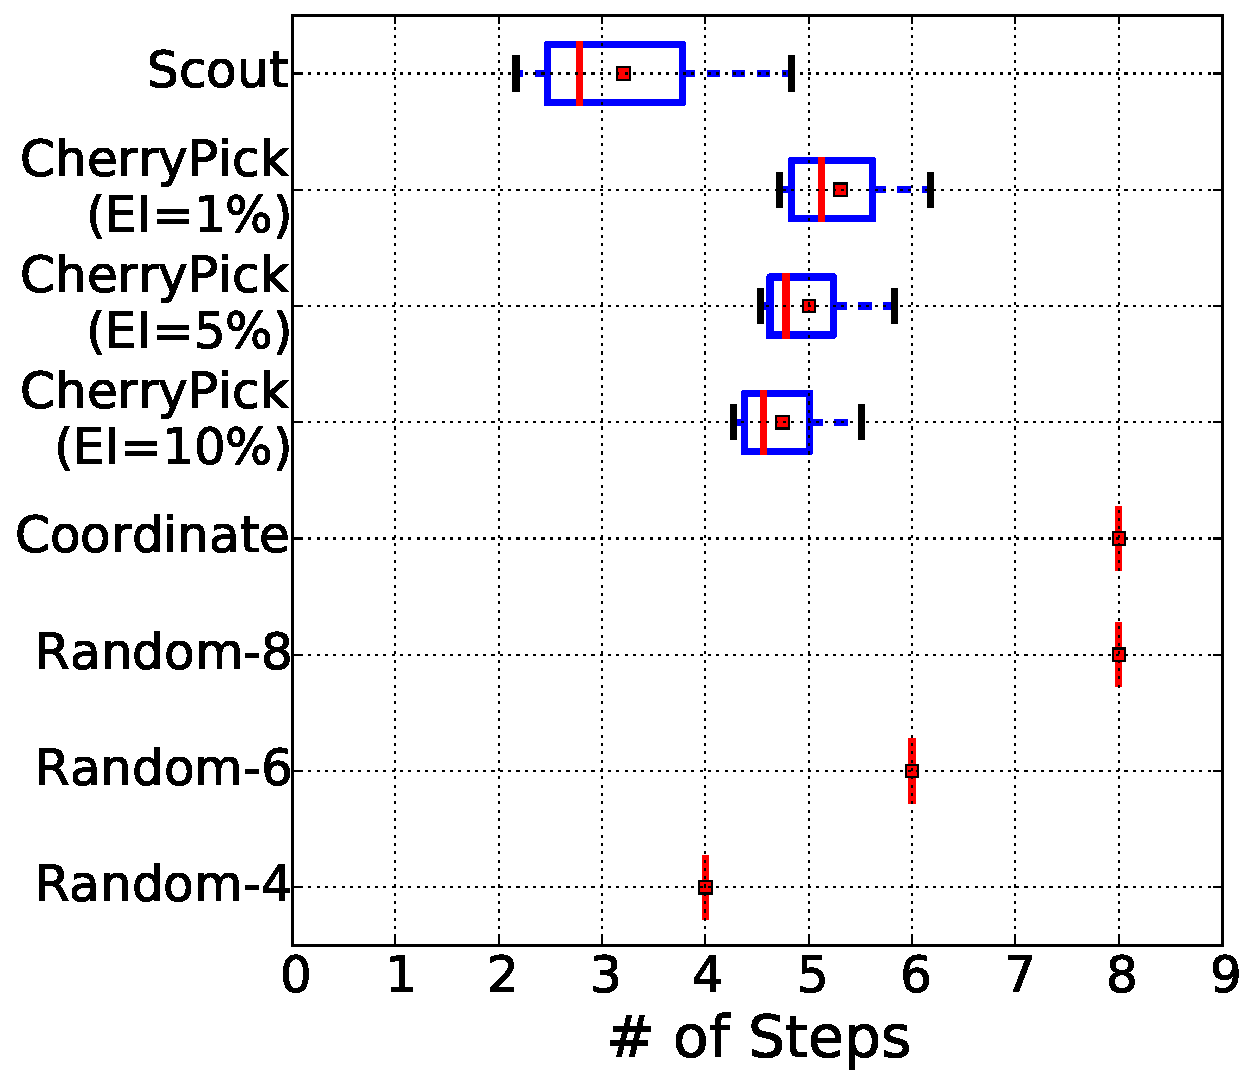
\includegraphics[width=\linewidth]{figures/single_time_overall_steps.pdf}
    \caption{Search Cost}
    \label{fig:single_time_overall_steps}
\end{subfigure}
\caption{\small{\textbf{Minimizing Execution Time.}
 The \emph{x-axis} represents the normalized performance (to the optimal configuration), and the optimal performance is $1$. 
 \scout finds the near-optimal solutions ($< 1.1$) in 87\% workloads while using much fewer steps.}}
\label{fig:single_time_overall}
\end{figure}


\subsubsection*{Deployment Choices}
Our evaluation examines both single- and multiple-node settings.
The single-node setting serves a comparison baseline and allows us to test more workloads (due to smaller search space).
In the single node setting,
we choose 18 distinct instance types or cloud configurations and 107 workloads.
When evaluating different cluster sizes,
we use strong scaling---fixed problem size---because we are interested in how to speed up a workload rather than the efficiency of the cluster.
For the multiple-node setting, we run 18 workloads
on 69 cloud configurations (9 instances with various cluster sizes).
%The search space is shown in~\myfigure{\ref{fig:search_space}}.

\subsubsection*{Dataset}
In order to verify the effectiveness of \scout,
we create a comprehensive performance data conversing all the combinations of
workloads and architectural configurations.
We collected our data on AWS.
\mytable{\ref{tab:dataset_overview}} present a summary.
Please refer to the open performance database for further details in Section~\ref{sec:cat::dataset}.


\subsubsection*{Parameters}
\scout has three important parameters:
1) labeled classes, 2) probability thresholds and 3) misprediction tolerance.
For the labeled classes in classification modeling,
we define five classes,
``better+'', ``better'',  ``fair'', ``worse'' and ``worse+'',
using thresholds [0.8, 0.95, 1.05, 1.2] as the cut points.
Regarding the two stopping criteria,
we choose $0.5$ for the probability threshold and
$3$ and $4$ for the misprediction tolerance
in the single-node and multiple-node setting respectively.
We examine the trade-off of these parameters in Section~\ref{sec:discussion}.

\subsection{Comparison Method}
To evaluate \scout, we examine the search performance
in terms of \emph{effectiveness}, \emph{efficiency} and \emph{reliability}.
We compare \scout with random search, coordinate descent, and \emph{CherryPick}.

\subsubsection*{Random search}
This search method
uniformly samples the configuration space.
The stopping criterion is the number of
configurations to evaluate.
A higher number yields better solution but also incurs higher search cost.
For a fair comparison, the search is repeated 100 times.  Random-4, -6, -8 represent random samples of 4, 6, and 8 cloud configurations respectively.
It serves as a na\"ive baseline method.


\begin{figure}[!htbp]
\centering
\begin{subfigure}[b]{0.4\textwidth}
    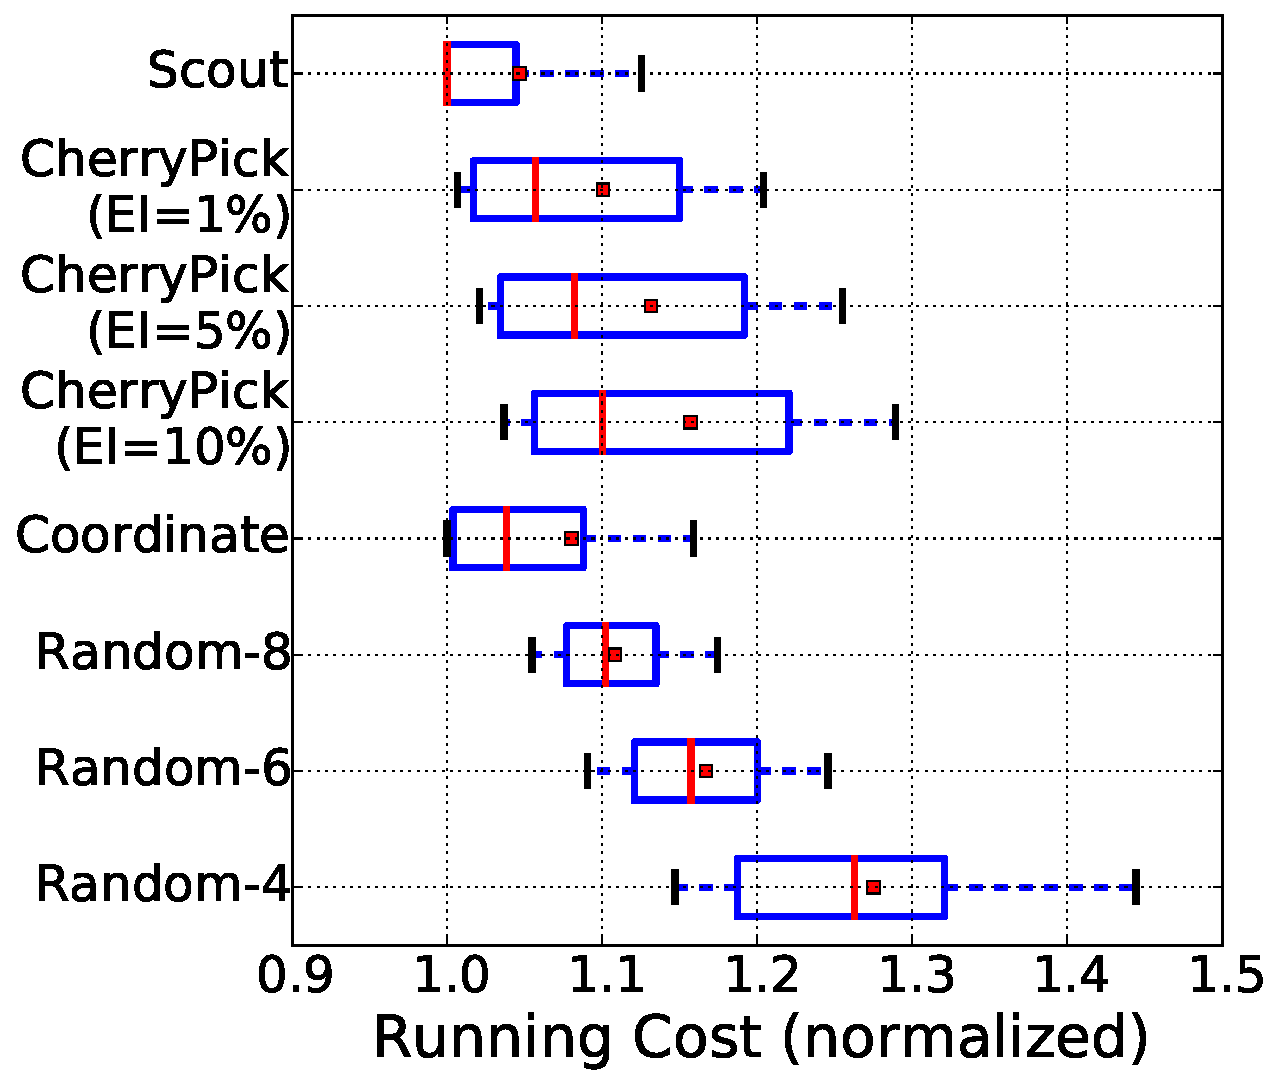
\includegraphics[width=\linewidth]{figures/single_cost_overall_performance.pdf}
    \caption{Search Performance}
    \label{fig:single_cost_overall_performance}
\end{subfigure}
\begin{subfigure}[b]{0.4\textwidth}
    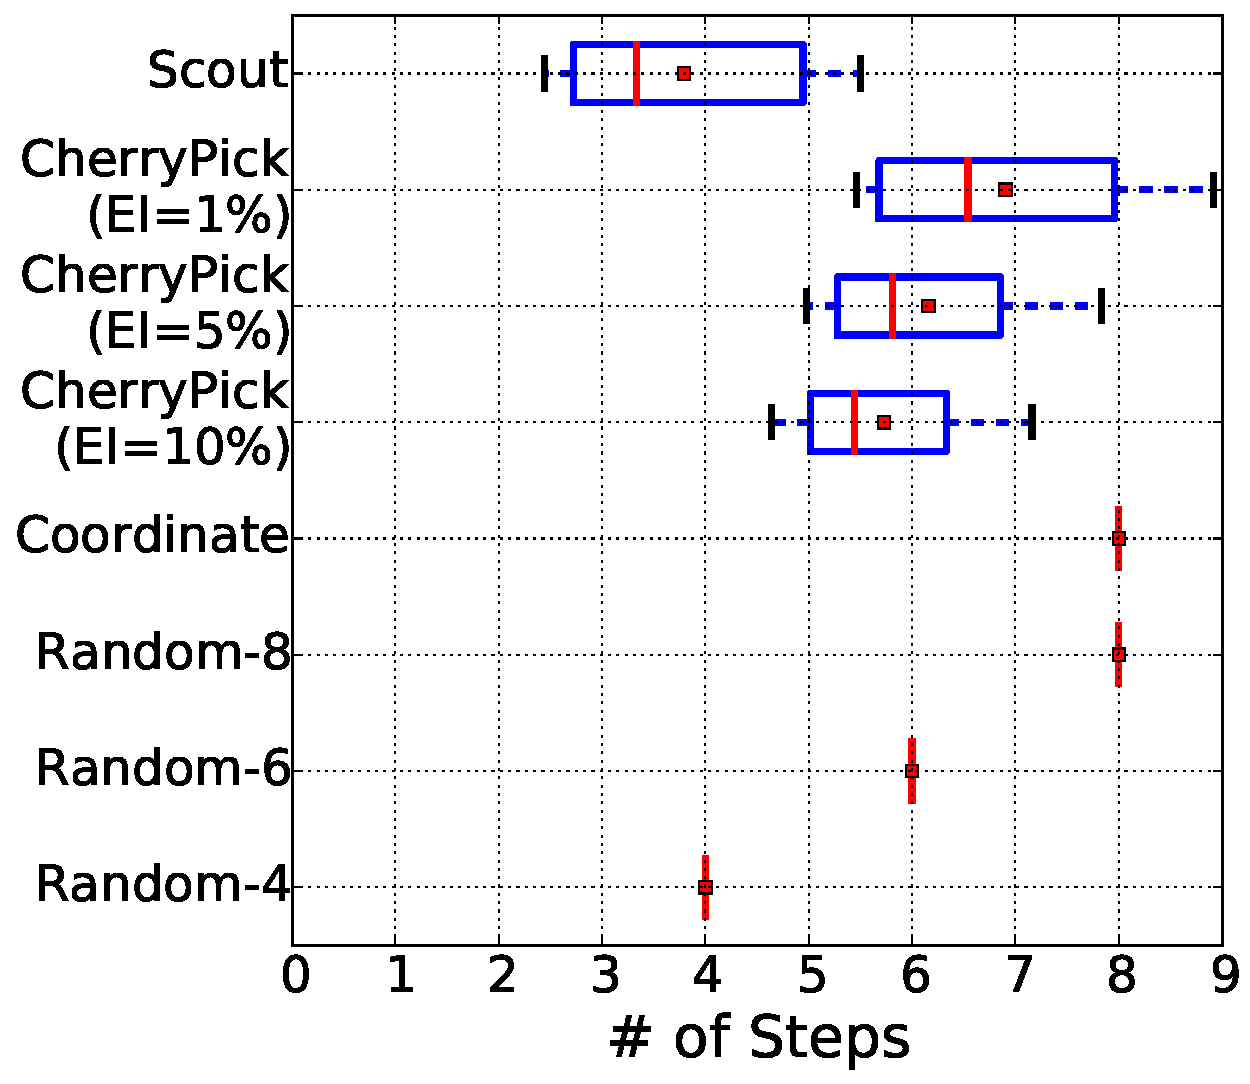
\includegraphics[width=\linewidth]{figures/single_cost_overall_steps.pdf}
    \caption{Search Cost}
    \label{fig:single_cost_overall_steps}
\end{subfigure}
\caption{\small{\textbf{Minimizing Running Cost.}
 Searching for the optimal cost is more difficult because the search cost is higher than the scenario of minimizing execution time. \scout still finds near-optimal solutions with a small increase in search cost while \emph{CherryPick} only finds near-optimal solutions in about 50\% workloads.}}
\label{fig:single_cost_overall}
\end{figure}


\subsubsection*{Coordinate descent}
This method searches
one dimension (\eg{CPU type and memory size}) at a time.
It determines the best choice of the dimension and
continues to choose the best from other dimensions.
This approach may suffer from local minimum due to
diminishing return and irregular performance outcome~\cite{Alipourfard2017}.
This situation worsens when the number of dimension increases.
In the evaluation, there are three dimensions:
(1) the instance family (such as \emph{c4} or \emph{r4}), (2)
the instance size (such as, \emph{large} or \emph{2xlarge}), and (3) the cluster size (the number of VMs).
The results are from 100 distinct searches, in which the starting point was randomly selected.


\subsubsection*{\cherrypick}
We implement the approach
proposed in \emph{CherryPick}~\cite{Alipourfard2017}.
We use
the same kernel function (\emph{Mat\'ern 5/2}) and
the same stopping criteria (\textbf{EI}=10\%).
We uniformly sample three configurations as starting points.
Since the search performance of \emph{CherryPick} is highly dependent on the selection of the starting points,
this experiment repeats 100 times to reduce artifacts
and give a better picture of \emph{CherryPick}'s capability.

We compare these approaches using three metrics.
First, we evaluate the effectiveness of the methods using
the \textit{normalized performance} (to the optimal choice).
It can be the \textit{execution time} or the \emph{deployment cost}.
Second, we use the search cost--- the number of cloud configurations measured to find the right cloud configuration.
% We consider the number of steps instead of the search cost (the total cost of actual measurements) because the former reveals how fast a method finds a solution.
Last, we examine how reliable our method is across the workloads. % (in single node setting) and 18 (in multiple-node setting).
We compare the aggregate of the normalized performance and the search cost along with their the 10\textsuperscript{th} and 90\textsuperscript{th} percentiles to observe whether our method performs well with consistency.  These numbers better illustrate reliability of the methods.


\begin{figure}[!htbp]
\centering
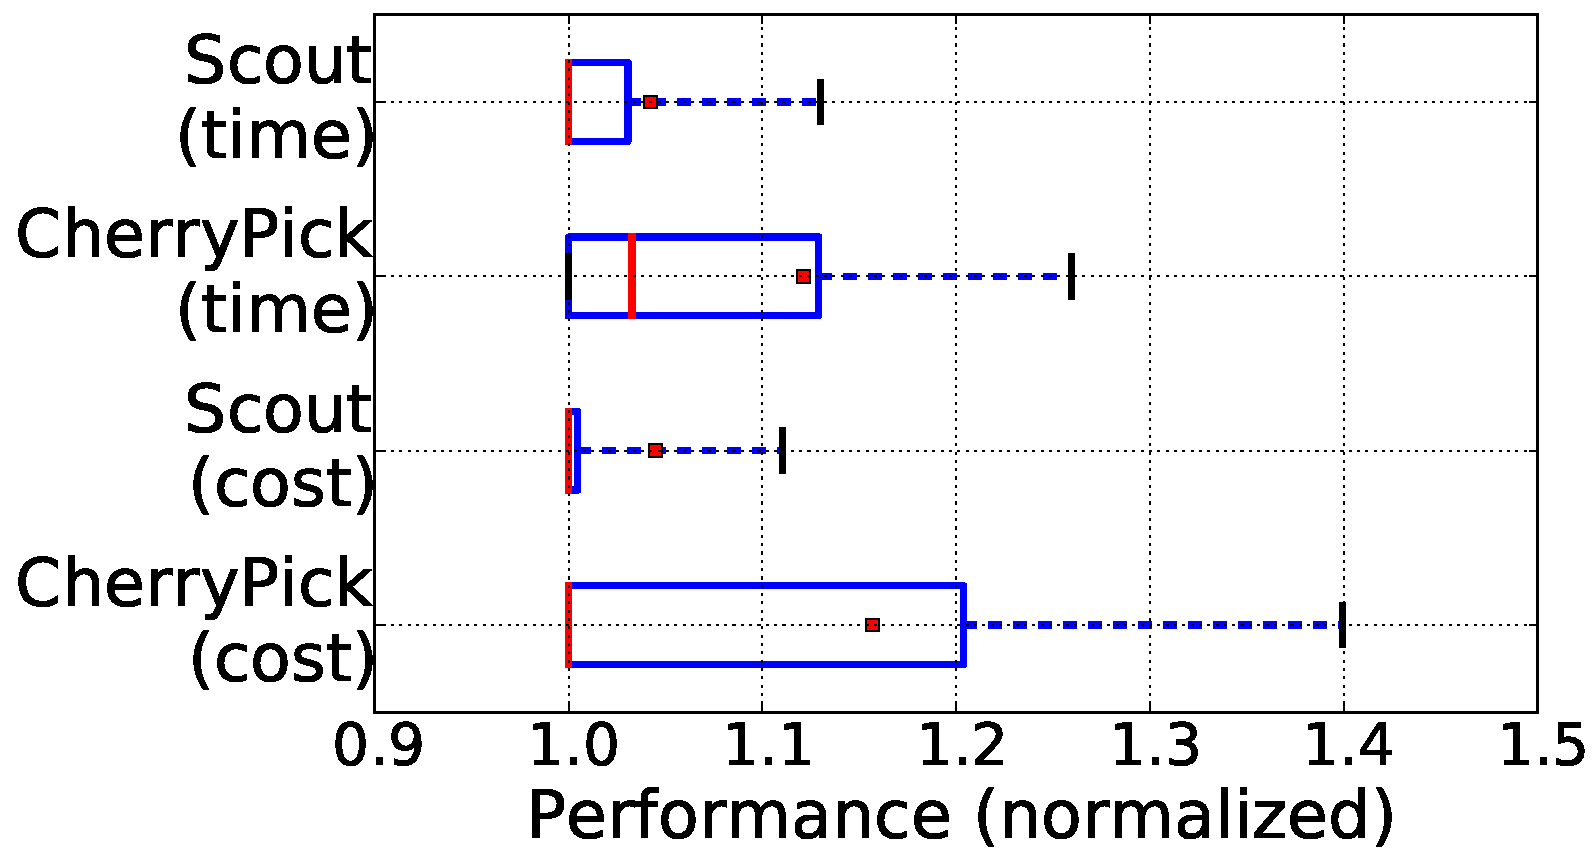
\includegraphics[width=0.6\textwidth]{figures/single_fragility.pdf}
\caption{\small{\textbf{Quality of found solutions.}
    Although both \emph{CherryPick} and \scout find the near optimal-solutions in most of the time,
    \scout is less fragile.}
}
\label{fig:single_fragility}
\end{figure}

\begin{figure}
\centering
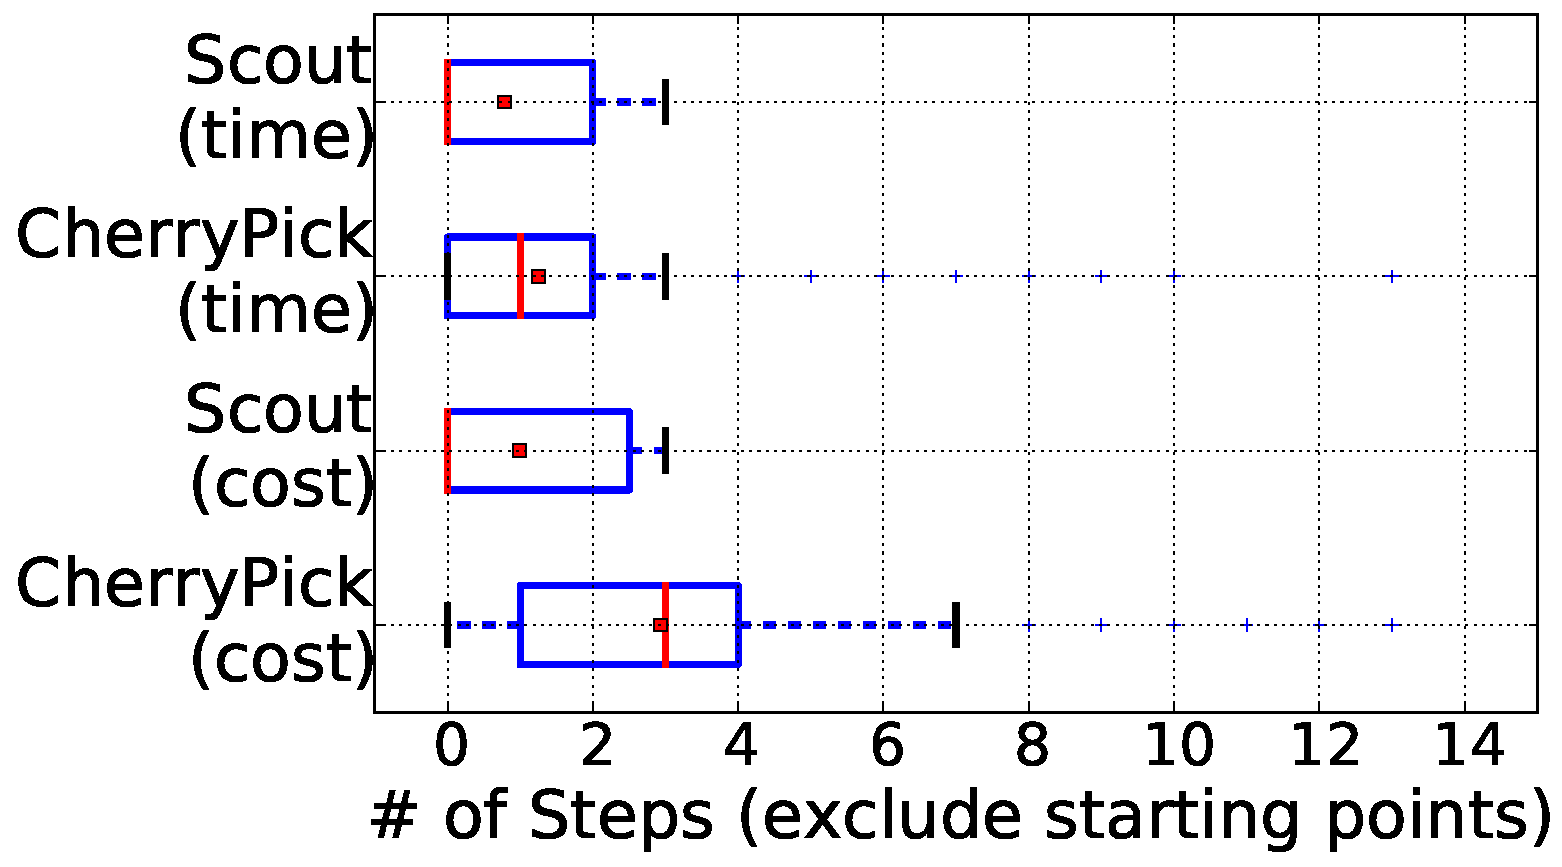
\includegraphics[width=0.6\textwidth]{figures/single_stopping_awareness.pdf}
\caption{\small{\textbf{Stopping awareness.}
    Search optimization avoids unnecessary search cost if it knows when the optimal solution is found.
    % \scout better acknowledges its existence.
    }}
\label{fig:single_startingpoint}

\end{figure}

\begin{figure}
\centering
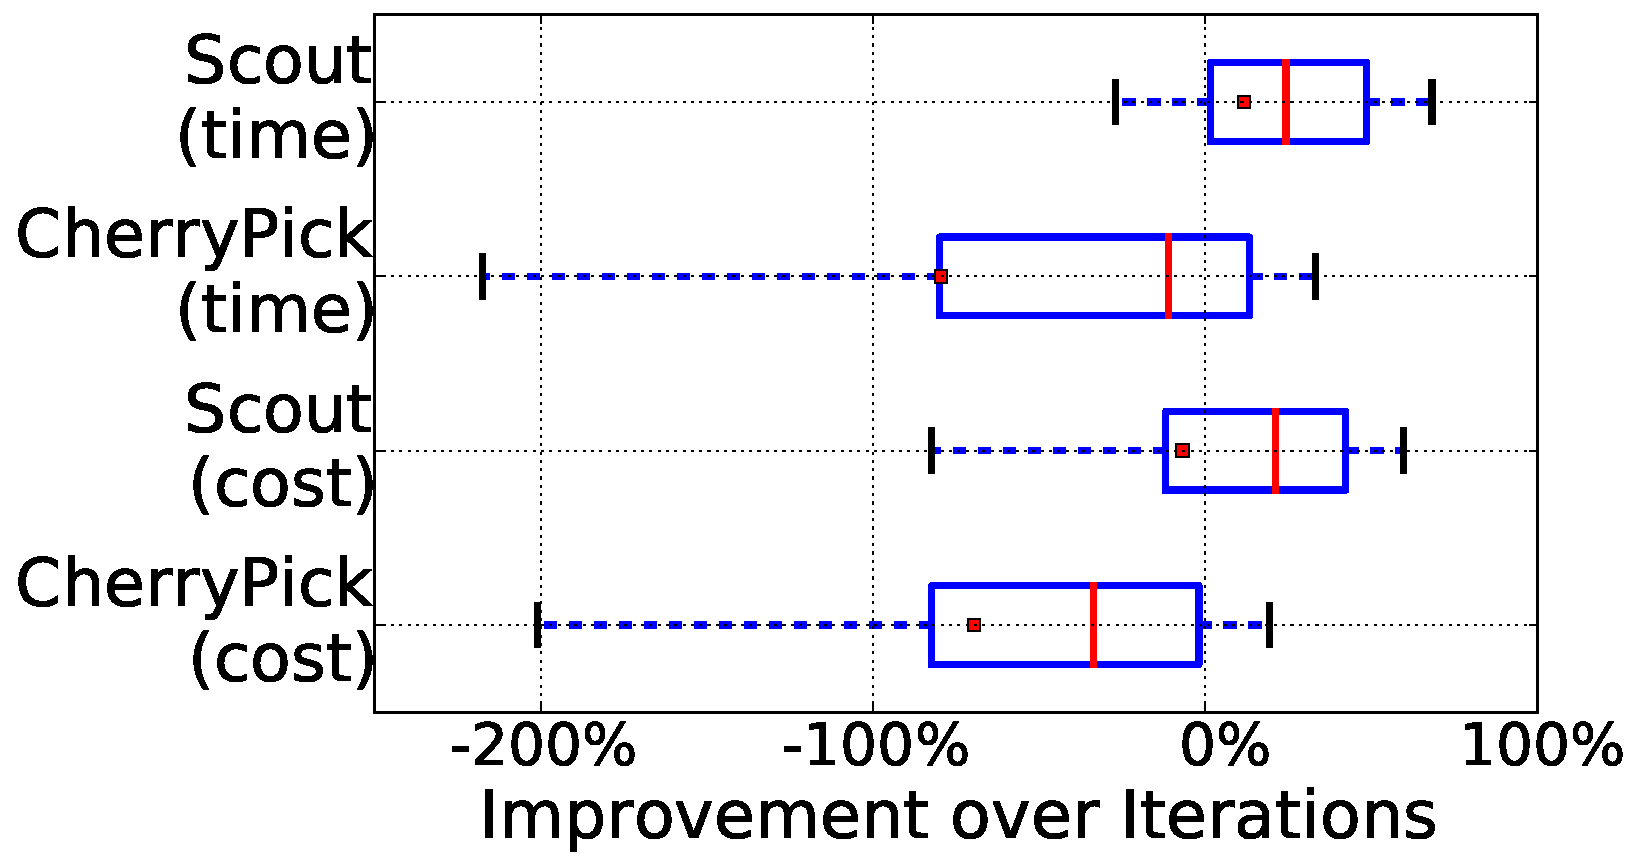
\includegraphics[width=0.6\textwidth]{figures/single_convergence.pdf}
\caption{\small{\textbf{Convergence speed.}
    \scout finds a better solution with 25\% improvement (on average) at each iteration, which suggests \scout is more likely to 
    converge.}}
\label{fig:search_convergence}
\end{figure}


\subsection{Is Scout effective and efficient?}

We examine search performance and search cost across 107 workloads in the single-node setting.
This evaluation largely answers whether a search method is reliable.

\textbf{Scout finds the near-optimal configurations
(within 10\% difference) for 87\% workloads}.
\myfigure{\ref{fig:single_time_overall_performance}} and \myfigure{\ref{fig:single_cost_overall_performance}} presents
the best cloud configuration (normalized to the optimal performance---1.0 represent the best, higher the worse) found by \scout and other methods while minimizing execution time and deployment cost, respectively. \myfigure{\ref{fig:single_time_overall_steps}} and \myfigure{\ref{fig:single_cost_overall_steps}} presents the search cost required the find the best cloud configuration which minimizes execution time and deployment cost, respectively. 
The figures display a box plot.
The box shows the inter-quartile range (from 25\textsuperscript{th} to 75\textsuperscript{th} percentile).
The vertical red line is the median, and the dot is the mean.
The whiskers to left and right show the 10\textsuperscript{th} and 90\textsuperscript{th} percentiles, respectively.
The horizontal axis shows execution time, and the vertical axis shows different techniques. 
An ideal search-based technique would find the best cloud configuration (in terms of performance) using the lower search cost.
These figures show the following.

\begin{itemize}[leftmargin=*]
    %\setlength\itemsep{-0.4em}
    \item \scout finds the best relative performance in terms of both execution time and deployment cost. The median performance of \scout, while searching for the cloud configuration which minimizes the deployment cost is 1.0, which means \scout was able to find the right cloud configuration.
    \item \scout is better than CherryPick across all measures (execution time, deployment cost, and search cost).
    \item \scout finds the best relative performance using the least search cost (fewer number of steps). Random-4 also requires low search cost, but its performance is much worse than \scout.
    \item The variance in the performance (in terms of execution time and deployment cost) of \scout is much lower than the other methods. The large variance of the Random methods can be attributed to their inherent randomness.
\end{itemize}


Overall, we see that \scout is that best performing method and \emph{CherryPick}, the state of the art method, only delivers similar performance in 64\% workloads while requiring 47\% greater search cost (4.7 compared to 3.2 steps). We also observe that the variance in the best cloud configuration found by \scout over 100 runs across 107 workloads is much lower than the other method. Hence, we can conclude that \scout is a reliable method to find the best cloud configuration.

\noindent\textbf{Cost creates a level playing field.}
Optimizing execution time is relatively easy
because a larger, more powerful instance type is more likely to have a shorter execution time.
However, the more powerful types are more expensive to execute.
Consequently, a smaller instance type may run longer but cost less.
Because the cost to execute an instance grow as the raw hardware performance increase, the differences in deployment cost between configurations tend to be much less than the differences between execution time.
This levels the playing field for cost---many more configurations are good candidates.
This leveling leads to, in general, longer searches,
as shown in \myfigure{\ref{fig:single_cost_overall_steps}}.
\emph{CherryPick} requires one extra step in optimizing deployment cost with a 15\% decrease of workloads in which it fails to find a solution within 10\% of the optimal configuration. To summarize, the performance of a search-based method is dependent on the objective of the search. From the data, we observe that searching for the best cloud configuration in terms of cost is more challenging than finding the best cloud configurations in terms of execution time. 




\subsection{Is \scout reliable?}
Users are willing to use a tool only when it is reliable. We evaluate the performance of \emph{CherryPick} and \scout
with different initial points for understanding their consistency.
In BO in \emph{CherryPick}, uses a random initial points to seed the search process and the effectiveness of CherryPick depend on these initial points. Selecting these initial points is non-trivial because (1) a good set of starting points for one workload does not work for other workloads, and (2) cloud providers frequently upgrade their instance portfolio with new instance types which make the process of selecting initial points more challenging. \scout is robust such that the effectiveness of \scout does not rely on initial points.


\begin{figure}[!htbp]
\centering
\begin{subfigure}[b]{0.4\textwidth}
    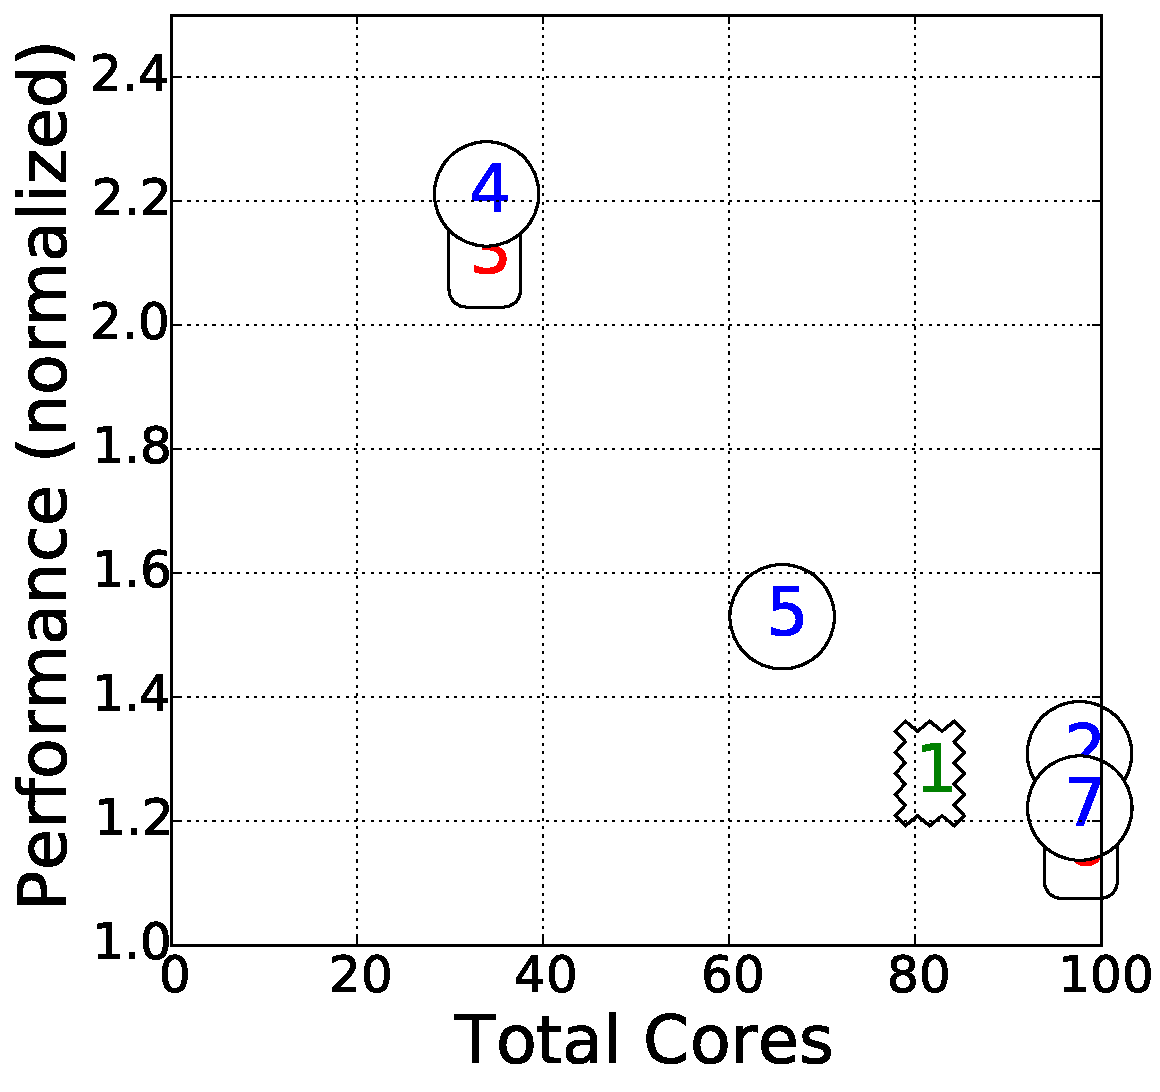
\includegraphics[width=\linewidth]{figures/multiple_bo_time_hadoop.pagerank.bigdata_12_cores.pdf}
    \caption{\cherrypick}
    \label{fig:comparison_time_cherrypick}
\end{subfigure}
\begin{subfigure}[b]{0.4\textwidth}
    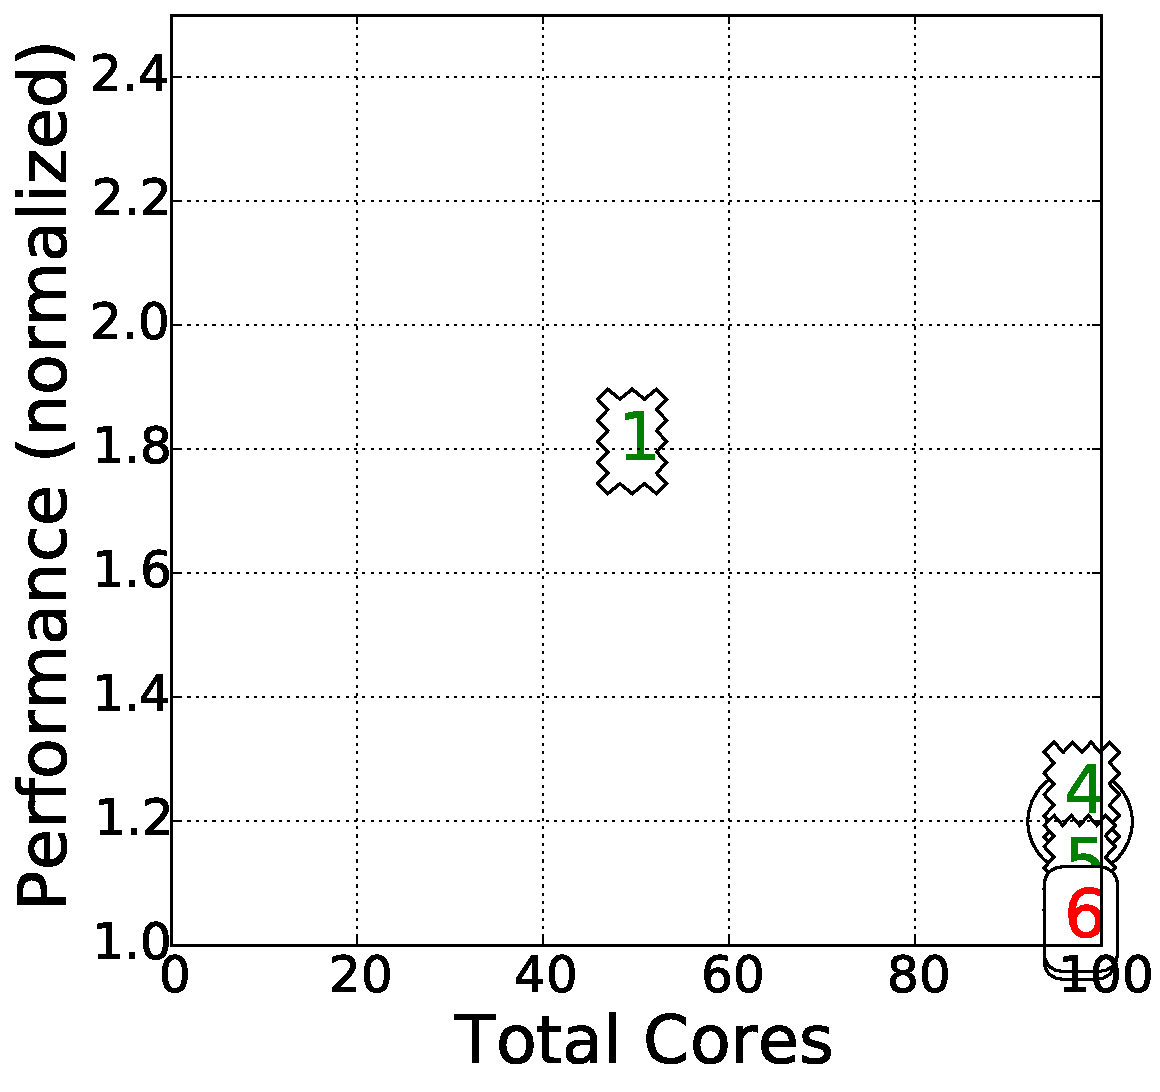
\includegraphics[width=\linewidth]{figures/multiple_scout_time_hadoop.pagerank.bigdata_24_m4.large_cores.pdf}
    \caption{\scout}
    \label{fig:comparison_time_scout}
\end{subfigure}
 \caption{\small{\textbf{Finding the fastest configuration for PageRank on Hadoop.} Left \& right sub-figure show the search path of CherryPick and \scout respectively. \scout identifies PageRank as a compute-intensive workload.  It chooses the configurations with higher core counts and CPU speed.}}
\label{fig:compare_1}
\end{figure}


To demonstrate the robustness of \scout, for each workload, we varied the initial points used in \emph{CherryPick}.
These points were randomly (without replacement) selected from the search space. On the other hand, \scout only needs one starting point, which is also selected randomly. This experiment was repeated 100 times to understand the implication of randomness.
\myfigure{\ref{fig:single_fragility}} shows the variance in the normalized performance of the found solutions by both the methods.
We see that 

\begin{itemize}[leftmargin=*]
    %\setlength\itemsep{-0.4em}
    \item \scout can find the optimal cloud configuration for most of the case since median performance is 1.0. However, there are some outliers which pushes the mean to 1.05. This is not a major concern since the 75$^{th}$ percentile is less than 1.05. This goes to show that the variance in the performance of 107 workloads aggregated over 100 runs is low.
    \item CherryPick is also effective in finding the cloud configuration since its median performance over 107 workloads is 1.05. We notice that the variance of the performance (both in terms of search performance and time) is larger than \scout. 
\end{itemize}


The variance in the results of CherryPick can be a major concern for the practitioners since a bad choice of initial points can lead to selecting either a slow or expensive configurations.
\scout, on the other hand, has more stable search performance regardless of the starting point.


\subsection{Why \scout works better?}
\label{sec:why_better}

\scout relies on quality routing policy to deliver good solutions.
We find \scout effective because
it knows when to stop searching and
converges to better solutions.

\begin{itemize}
\item \textbf{\scout knows when to stop.}
When an optimizer can stop as soon as it finds the optimal solution (or near-optimal solutions),
it can avoid unnecessary search efforts. \myfigure{\ref{fig:single_startingpoint}} shows that \scout requires a fewer number of steps if the starting point is already the optimal configuration.

\item \textbf{Convergence speed.}
The speed of convergence of a search-based method is dependent how it selects the next cloud configuration to measure. An ideal search-based method will always find the next cloud configuration, which is better than the cloud configurations sampled previously. \textit{Converge speed} can be defined as the average difference between the performance score (execution time or deployment cost) of the previous measurement (i$^{th}$ step) and the current measurement (i+1$^th$ step). A positive number would indicate that the current cloud configuration is better than the previous measurement (for both deployment cost and execution time, lower is better). \myfigure{\ref{fig:search_convergence}} compares the convergence speed of CherryPick and \scout. \myfigure{\ref{fig:search_convergence}} indicates that \scout overall finds cloud configurations 50\% (median) better execution time than the current cloud configuration, whereas CherryPick overall moves to cloud configuration which is 25\% worse than the current best configuration. Similar behavior is seen for deployment cost. This is evidence to show that \scout uses the historical data to find the promising region in the search space and exploits that space effectively.

\end{itemize}



\begin{figure}[!htbp]
\centering
\begin{subfigure}[b]{0.4\textwidth}
    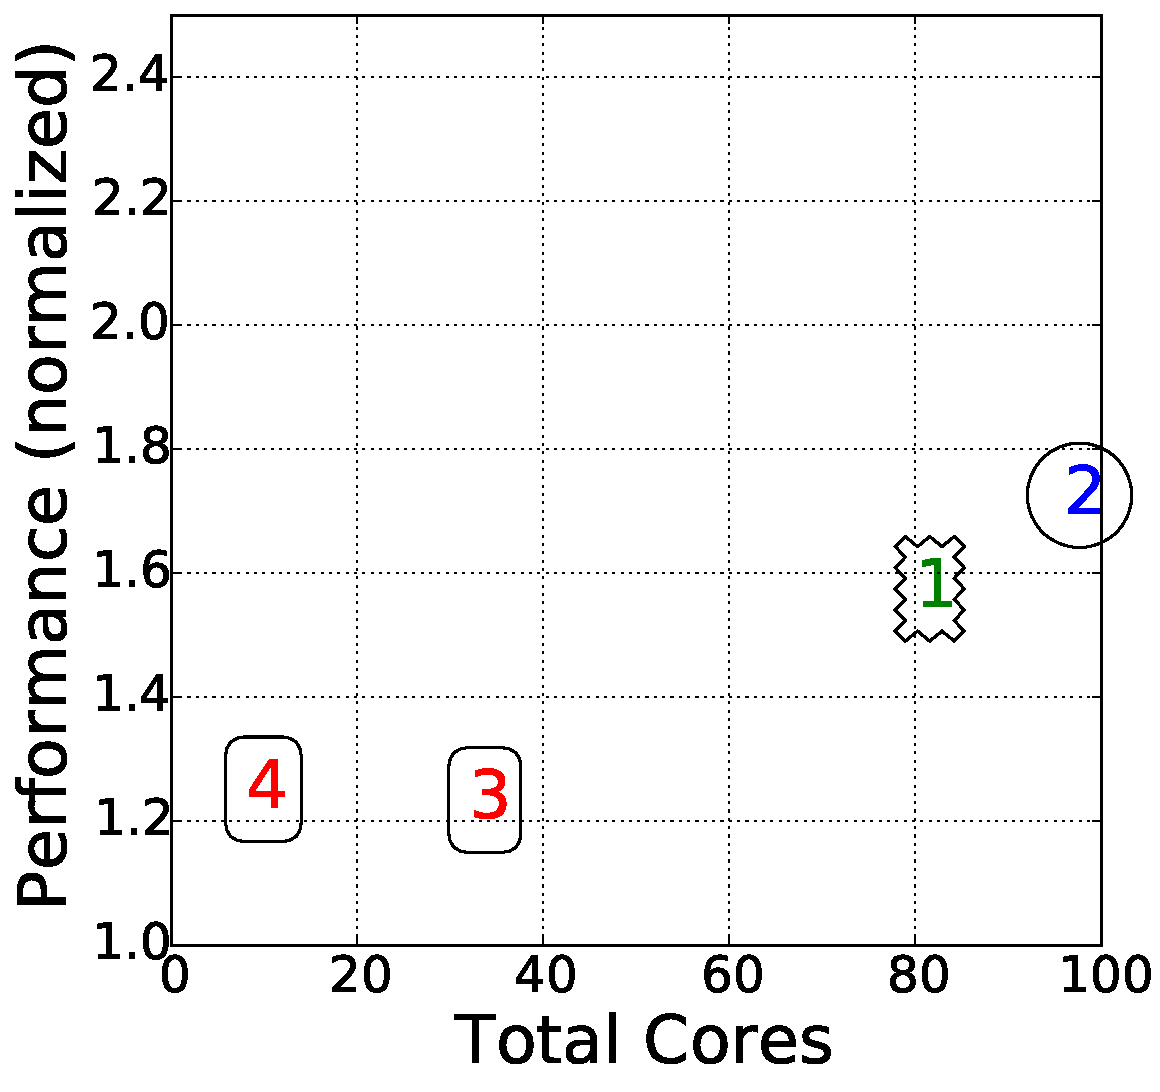
\includegraphics[width=\linewidth]{figures/multiple_bo_cost_spark1.5.naive-bayes.huge_12_cores.pdf}
    \caption{\cherrypick}
    \label{fig:comparison_cost_cherrypick}
\end{subfigure}
\begin{subfigure}[b]{0.4\textwidth}
    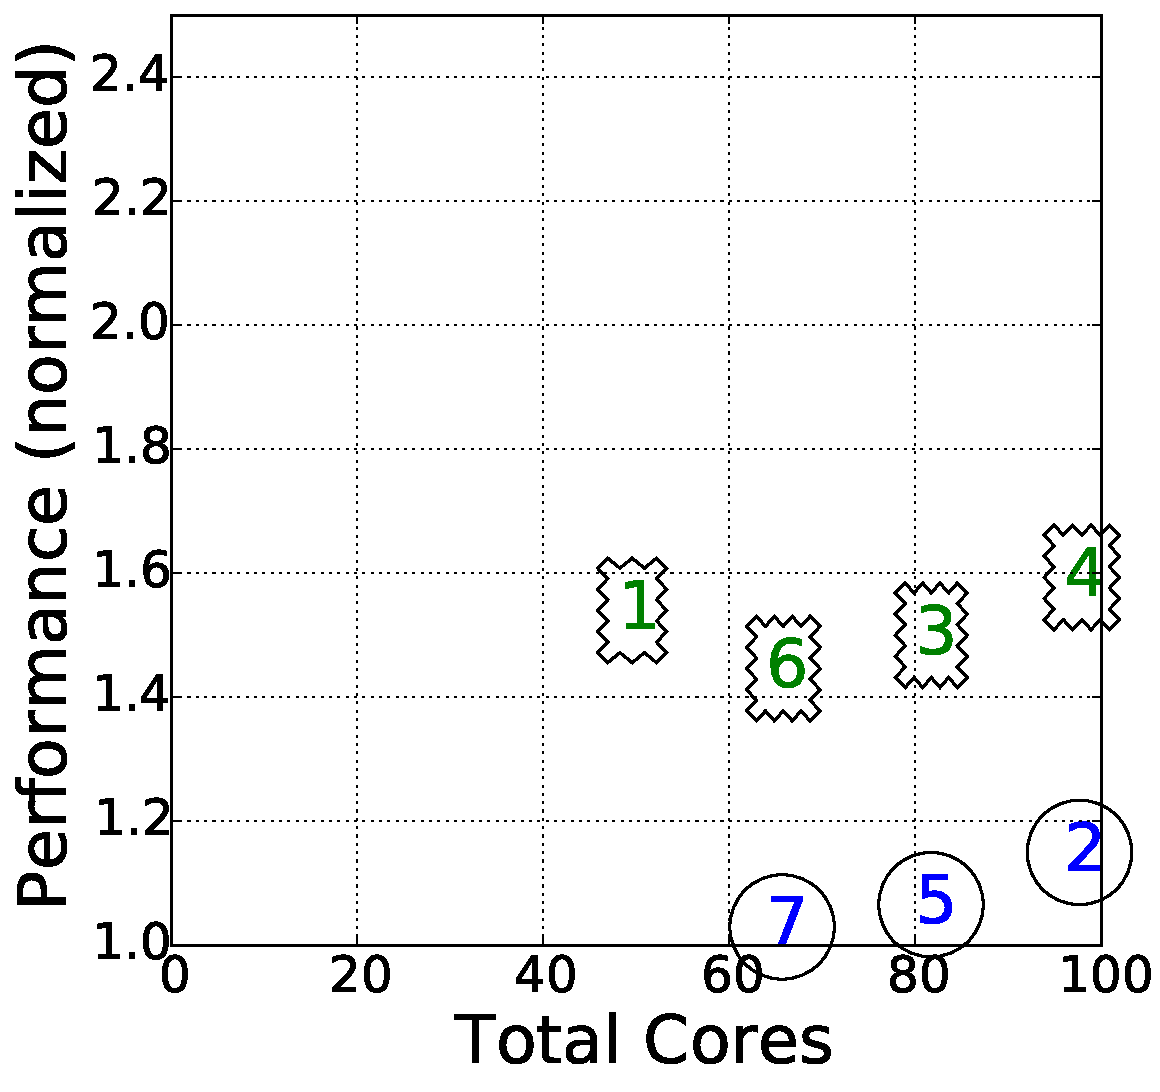
\includegraphics[width=\linewidth]{figures/multiple_scout_cost_spark1.5.naive-bayes.huge_24_m4.large_cores.pdf}
    \caption{\scout}
    \label{fig:comparison_cost_scout}
\end{subfigure}
\caption{\small{\textbf{Minimizing the running cost for Naive-Bayes on Spark.} This is a memory-intensive workload.  \scout does not even try the \emph{c4} family due to its small memory per core.}}
\label{fig:compare_4}
\end{figure}



\subsection{Example Search Process}

This section compares and contrasts the properties of \emph{CherryPick} and \scout.
We provides four examples of optimizing execution time (in Figure~\ref{fig:compare_1} and~\ref{fig:compare_2}) and running cost (in Figure~\ref{fig:compare_3} and~\ref{fig:compare_1}). Different colored markers in the graphs represent different families of instances: \textcolor{green}{green} represent the m4 family---general purpose, \textcolor{blue}{blue} represent the r4 family---memory optimized, and \textcolor{red}{red} represent the c4 family---compute optimized.
We evaluate \emph{CherryPick} and \scout on four representative workloads, selected based on diverse resource requirements (CPU intensive, Memory intensive).
For \emph{CherryPick}, we choose
\emph{20$\times$m4.xlarge}, \emph{48$\times$r4.large} and \emph{16$\times$c4.large} as the starting points because
they are wide spread in the search space.
Since \scout only needs one starting point,
we choose \emph{24$\times$m4.large} because it is the mid point of the search space.
We observe that \emph{CherryPick} can find near-optimal solutions for few workloads if not all.

\begin{figure}[!htbp]
\centering
\begin{subfigure}[b]{0.4\textwidth}
    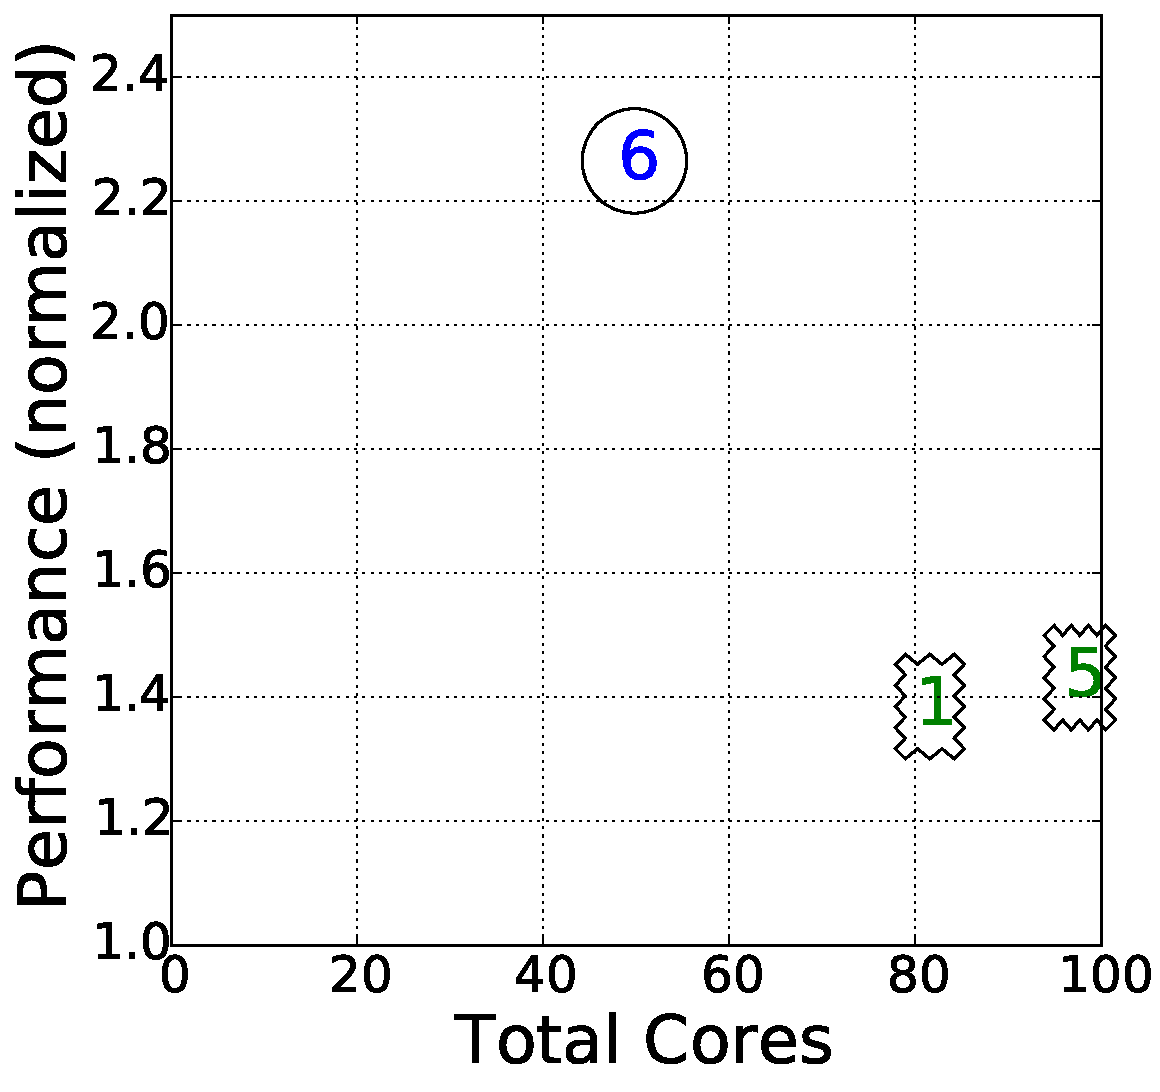
\includegraphics[width=\linewidth]{figures/multiple_bo_time_spark1.5.regression.huge_12_cores.pdf}
    \caption{\cherrypick}
    \label{fig:search_time_cherrypick}
\end{subfigure}
\begin{subfigure}[b]{0.4\textwidth}
    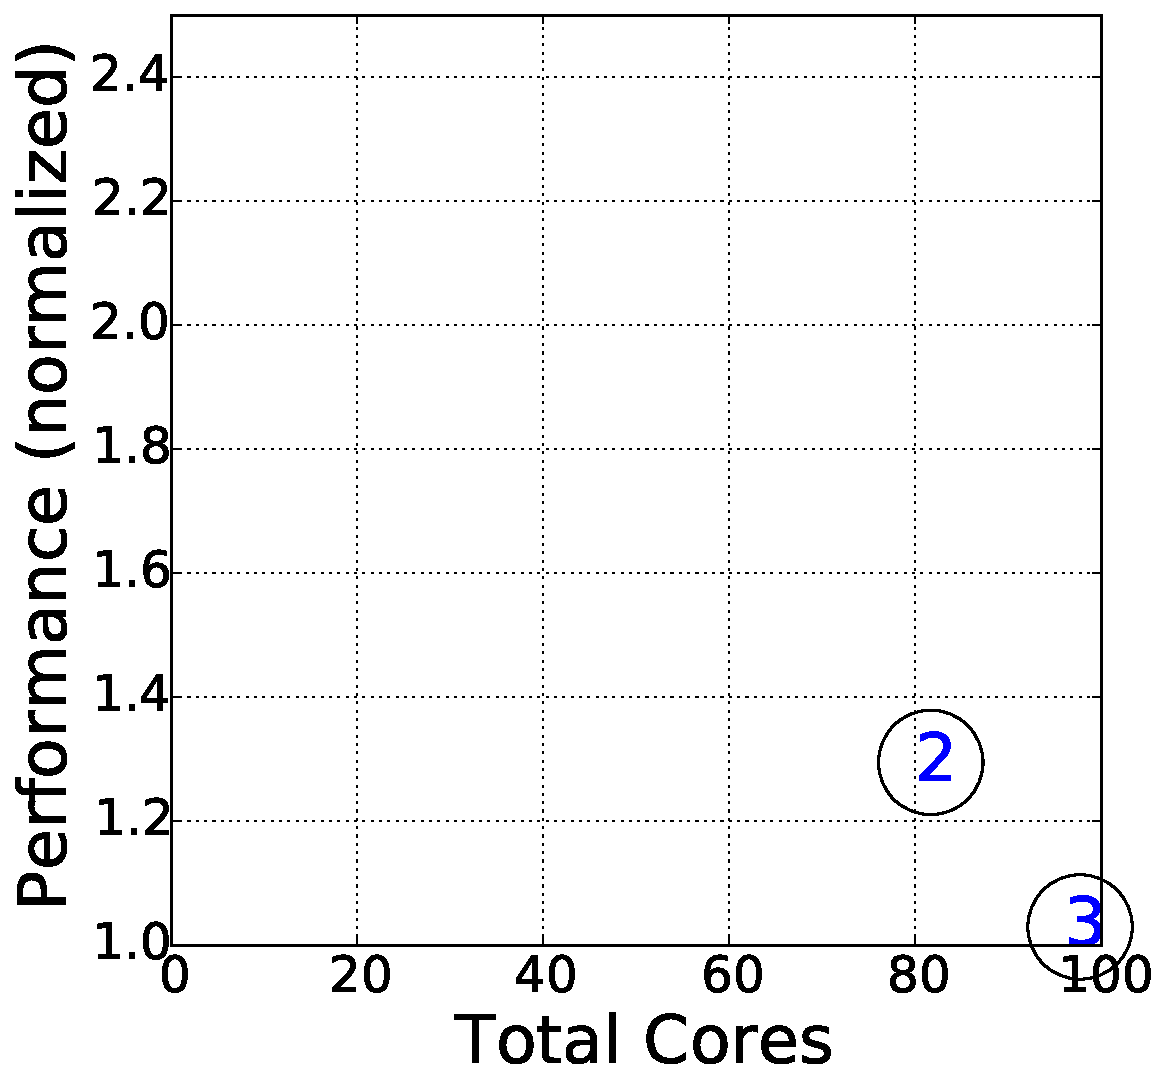
\includegraphics[width=\linewidth]{figures/multiple_scout_time_spark1.5.regression.huge_24_m4.large_cores.pdf}
    \caption{\scout}
    \label{fig:search_time_scout}
\end{subfigure}
\caption{\small{\textbf{Minimizing execution time of Regression on Spark.} Since the Regression workload requires both computation and large memory, \scout directly chooses configurations with the \emph{r4} family and larger cores.}}
\label{fig:compare_2}
\end{figure}

\subsubsection*{Reliable exploration is difficult and generates high search cost}
In Figure~\ref{fig:compare_2},~\ref{fig:compare_3},~\ref{fig:compare_1},~\ref{fig:compare_4}, we observe that the search path generated by \emph{CherryPick} involves more distinct VM types due to the need to explore the performance model. For example, in Figure~\ref{fig:compare_3}, CherryPick visits each instance family at once in all examples while \scout skips some specific families.
This is because \scout builds the performance model from historical data. Hence, it requires only little (or no) exploration. This phenomenon, exploration-exploitation dilemma, is studied extensively in Machine learning~\cite{kaelbling1996reinforcement}. The cold-start issue (as described in Section~\ref{sec:motivation} arises partly because of the requirement to explore the configuration space since \scout learns the performance behavior from historical data from workloads (previously explored) can sidestep the need to explore the search space.




\subsubsection*{Fragility of CherryPick}
As explained in Section~\ref{sec:motivation}, CherryPick is fragile
because it is sensitive to its parameters and the starting points.
In the four examples, \emph{CherryPick} starts from the same three configurations; however, the results are very different.
In \myfigure{\ref{fig:compare_3}}, \emph{CherryPick} fails to characterize the search space, which results in long search path (and high search cost).
While in \myfigure{\ref{fig:compare_4}},
\emph{CherryPick} stops too early and only finds a local minima (the $c4$ family).
These two examples show that \emph{CherryPick} is fragile and therefore, its search performance is not stable.

\subsubsection*{\scout identifies resource requirements}
When resource requirements can be articulated, a search process is more likely to find cloud configurations effectively and efficiently. In \myfigure{\ref{fig:compare_1}},
the \emph{PageRank} workload runs faster on a larger cluster (higher core counts) and higher-frequency CPUs. The \emph{r4} family, with larger memory but slower CPU speed, does not seem to be the best choice, hence avoided by \scout and instead prefers \emph{c4} and \emph{m4} family.
This tendency is more clear in the other cases as well (Figure~\ref{fig:compare_2}, ~\ref{fig:compare_3}, and~\ref{fig:compare_4}).


\begin{figure}[!htbp]
\centering
\begin{subfigure}[b]{0.4\textwidth}
    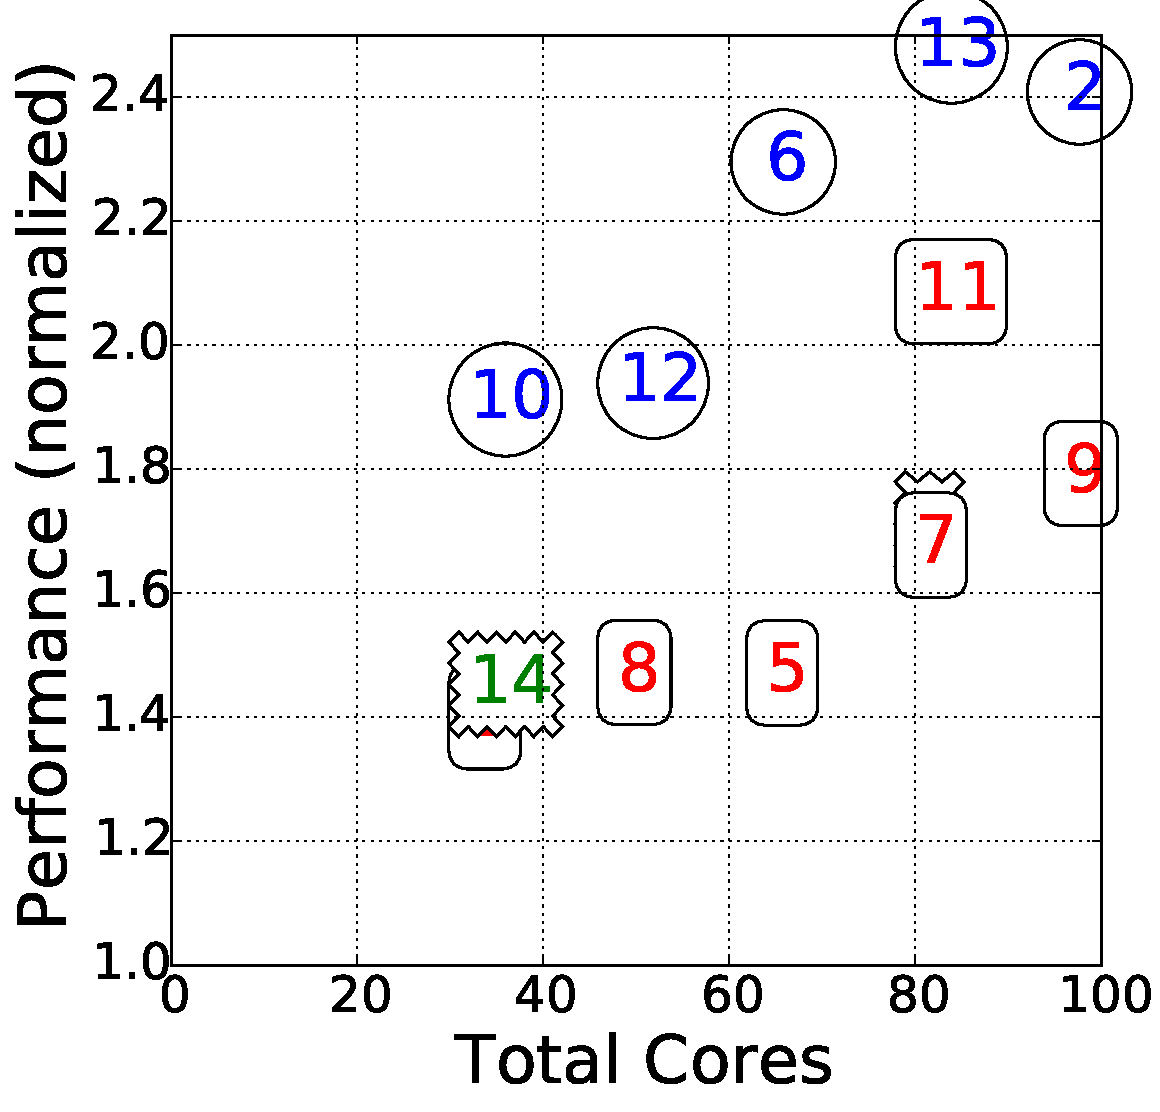
\includegraphics[width=\linewidth]{figures/multiple_bo_cost_hadoop.terasort.bigdata_12_cores.pdf}
    \caption{\cherrypick}
    \label{fig:search_cost_cherrypick}
\end{subfigure}
\begin{subfigure}[b]{0.4\textwidth}
    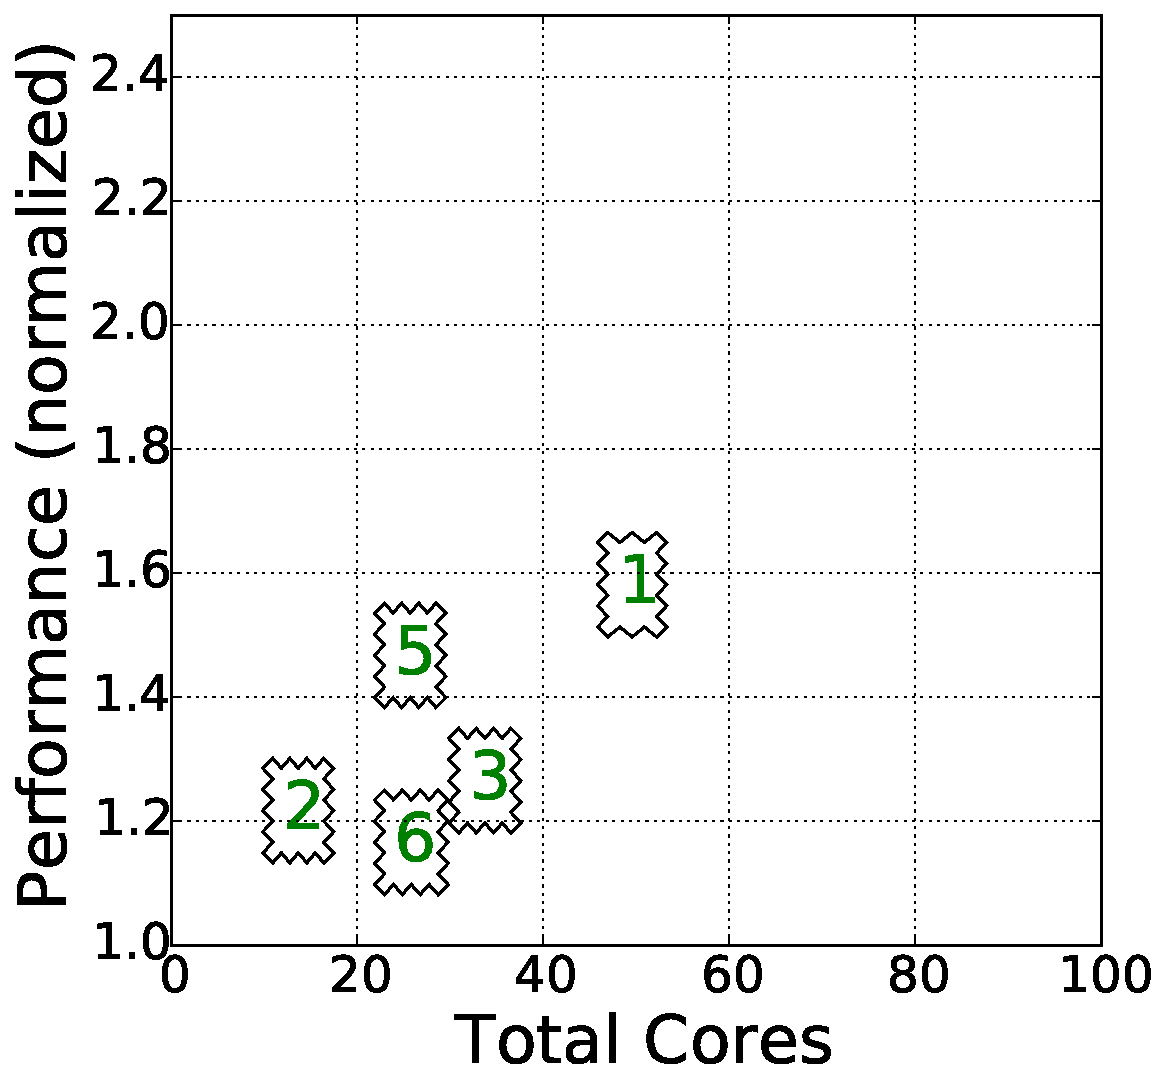
\includegraphics[width=\linewidth]{figures/multiple_scout_cost_hadoop.terasort.bigdata_24_m4.large_cores.pdf}
    \caption{\scout}
    \label{fig:search_cost_scout}
\end{subfigure}
\caption{\small{\textbf{Finding the cheapest configuration for Terasort on Hadoop.} The Terasort workload requires enough memory to avoid spilling data to disks. Besides, a large cluster can be insufficient due to the shuffle phase in MapReduce.  \scout chooses a smaller cluster with the general-purpose VM type. }}
\label{fig:compare_3}
\end{figure}



\subsubsection*{\scout captures the complex cost model}
In a real-world setting, practitioners can choose either a smaller cluster built using more powerful instances or choose large cluster built using smaller or less powerful instances (a scale-out and a scale-out configuration). The performance model used by \scout can infer the size of the cluster of the best cloud configuration.
In \myfigure{\ref{fig:compare_3}}, \scout chooses to run \emph{TeraSort} on a smaller cluster to save cost. On the contrary, in Figure~\ref{fig:compare_4}, \scout selects a larger cluster for efficiently running the \emph{Naive-Bayes} workload while achieving lower cost. These two examples show that \scout captures the complex relationship between the resource metrics and the running cost.


\subsubsection*{Summary}
The main difference between \emph{CherryPick} and \scout lies how the method explores the space of possible cloud configuration options. We can see that \emph{CherryPick} has to explore more cloud configuration options and hence have higher search cost (longer search path) while \scout searches within a relatively restricted region. This feature of \scout can be attributed to its performance model, which learns from the historical data. This also goes to show that encoding scheme, which uses low-level performance metrics, is successful in transferring knowledge from one workload to another.


